
        \documentclass[spanish, 11pt]{exam}

        %These tell TeX which packages to use.
        \usepackage{array,epsfig}
        \usepackage{amsmath, textcomp}
        \usepackage{amsfonts}
        \usepackage{amssymb}
        \usepackage{amsxtra}
        \usepackage{amsthm}
        \usepackage{mathrsfs}
        \usepackage{color}
        \usepackage{multicol, xparse}
        \usepackage{verbatim}


        \usepackage[utf8]{inputenc}
        \usepackage[spanish]{babel}
        \usepackage{eurosym}

        \usepackage{graphicx}
        \graphicspath{{../img/}}
        \usepackage{pgf}



        \printanswers
        \nopointsinmargin
        \pointformat{}

        %Pagination stuff.
        %\setlength{\topmargin}{-.3 in}
        %\setlength{\oddsidemargin}{0in}
        %\setlength{\evensidemargin}{0in}
        %\setlength{\textheight}{9.in}
        %\setlength{\textwidth}{6.5in}
        %\pagestyle{empty}

        \let\multicolmulticols\multicols
        \let\endmulticolmulticols\endmulticols
        \RenewDocumentEnvironment{multicols}{mO{}}
         {%
          \ifnum#1=1
            #2%
          \else % More than 1 column
            \multicolmulticols{#1}[#2]
          \fi
         }
         {%
          \ifnum#1=1
          \else % More than 1 column
            \endmulticolmulticols
          \fi
         }
        \renewcommand{\solutiontitle}{\noindent\textbf{Sol:}\enspace}

        \newcommand{\samedir}{\mathbin{\!/\mkern-5mu/\!}}

        \newcommand{\class}{1º Bachillerato}
        \newcommand{\examdate}{\today}

        \newcommand{\tipo}{A}


        \newcommand{\timelimit}{50 minutos}



        \pagestyle{head}
        \firstpageheader{
\includegraphics[width=0.2\columnwidth]{header_left}}{\textbf{Departamento de Matemáticas\linebreak \class}\linebreak \examnum}{
\includegraphics[width=0.1\columnwidth]{header_right}}
        \runningheader{\class}{\examnum}{Página \thepage\ of \numpages}
        \runningheadrule

        \newcommand{\examnum}{31 - Funciones}
        \begin{document}
        \begin{questions}
        \question p65e06-0 - Halla el dominio de las siguientes funciones: 
    
        \begin{multicols}{1}
        \begin{parts} \part[1] $f(x)=0x-3$  \begin{solution}   $Dom\left(f \right)=\mathbb{R}$   \end{solution} \part[1] $f(x)=x^3-5x^2+2$  \begin{solution}   $Dom\left(f \right)=\mathbb{R}$   \end{solution} \part[1] $f(x)=\frac{{x - 1}}{{x + 5}}$  \begin{solution}   $Dom\left(f \right)=\left(-\infty, -5\right) \cup \left(-5, \infty\right)$   \end{solution} \part[1] $f(x)=7x-1$  \begin{solution}   $Dom\left(f \right)=\mathbb{R}$   \end{solution} \part[1] $f(x)=\frac{2}{x}$  \begin{solution}   $Dom\left(f \right)=\left(-\infty, 0\right) \cup \left(0, \infty\right)$   \end{solution} \part[1] $f(x)=\sqrt[3]{\frac{x + 1}{x - 2}}$  \begin{solution}   $Dom\left(f \right)=\left(-\infty, 2\right) \cup \left(2, \infty\right)$   \end{solution} \part[1] $f(x)=\sqrt {{x^2} - 9}$  \begin{solution}   $Dom\left(f \right)=\left(-\infty, -3\right] \cup \left[3, \infty\right)$   \end{solution} \part[1] $f(x)=\sqrt {x+3}$  \begin{solution}   $Dom\left(f \right)=\left[-3, \infty\right)$   \end{solution}
        \end{parts}
        \end{multicols}
        \question p65e17-0 - Dadas las funciones $f(x)= x^2+5$, $g(x)= \frac{{x - 1}}{{x + 3}}$ y $h(x)= \sqrt{x}$. Calcula: 
    
        \begin{multicols}{1}
        \begin{parts} \part[1] $g \circ f$  \begin{solution}   $g{\left (f{\left (x \right )} \right )}=\frac{x^{2} + 4}{x^{2} + 8}$   \end{solution} \part[1] $f \circ g$  \begin{solution}   $f{\left (g{\left (x \right )} \right )}=\frac{\left(x - 1\right)^{2}}{\left(x + 3\right)^{2}} + 5$   \end{solution} \part[1] $h \circ g \circ f$  \begin{solution}   $h{\left (g{\left (f{\left (x \right )} \right )} \right )}=\frac{\sqrt{x^{2} + 4}}{\sqrt{x^{2} + 8}}$   \end{solution}
        \end{parts}
        \end{multicols}
        \question p66e23y24 - Halla la función inversa de $f(x)$, y comprueba el resultado, siendo:
        \begin{multicols}{1}
        \begin{parts} \part[1] $f(x)=3 x - 2$  \begin{solution}   $f^{-1}(x)=\frac{x}{3} + \frac{2}{3}$ \\ $f^{-1} \circ f(x)=x=x$ \\\\ \resizebox{0.4\textwidth}{!}{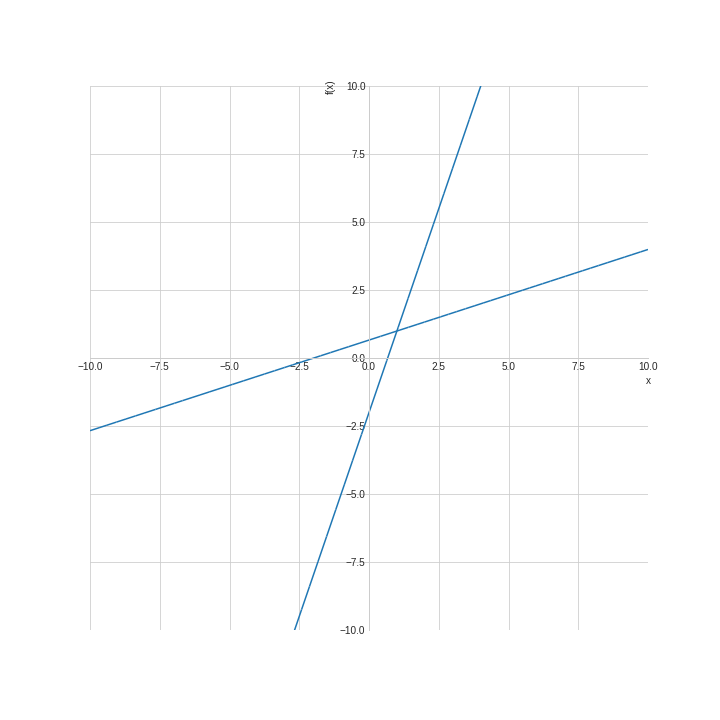
\includegraphics[width=1\columnwidth]{p66e23y24-0}}   \end{solution} \part[1] $f(x)=\frac{x + 2}{- x + 1}$  \begin{solution}   $f^{-1}(x)=\frac{x - 2}{x + 1}$ \\ $f^{-1} \circ f(x)=\frac{-2 + \frac{x + 2}{- x + 1}}{1 + \frac{x + 2}{- x + 1}}=x$ \\\\ \resizebox{0.4\textwidth}{!}{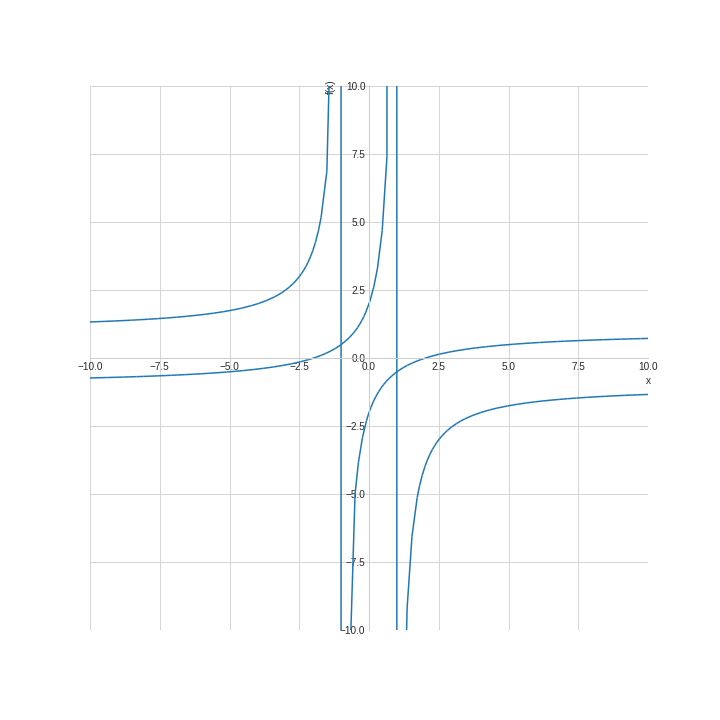
\includegraphics[width=1\columnwidth]{p66e23y24-1}}   \end{solution}
        \end{parts}
        \end{multicols}
        \question p68e28 - Representa gráficamente las siguientes funciones:
        \begin{multicols}{1}
        \begin{parts} \part[1] $y=-5x$  \begin{solution}   \\ \resizebox{0.4\textwidth}{!}{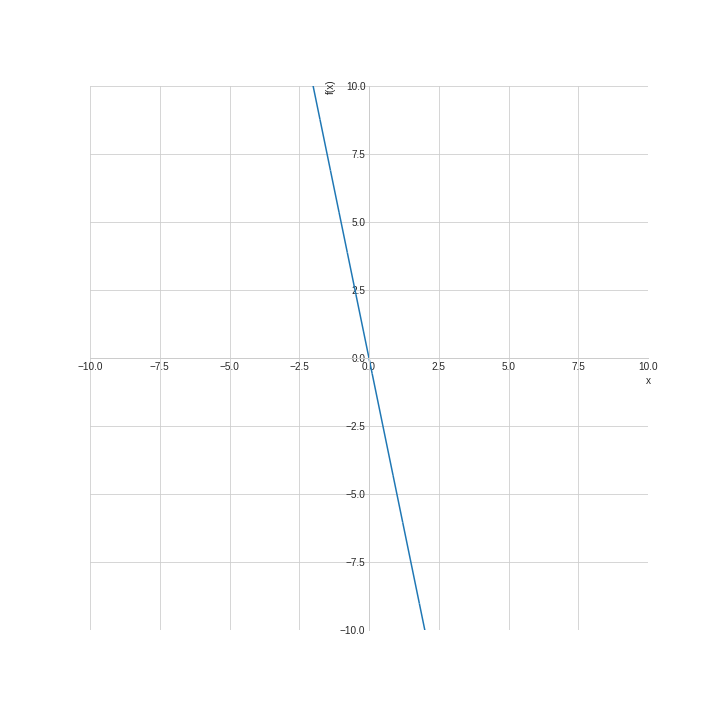
\includegraphics[width=1\columnwidth]{p68e28-0}}   \end{solution} \part[1] $y=-5x+3$  \begin{solution}   \\ \resizebox{0.4\textwidth}{!}{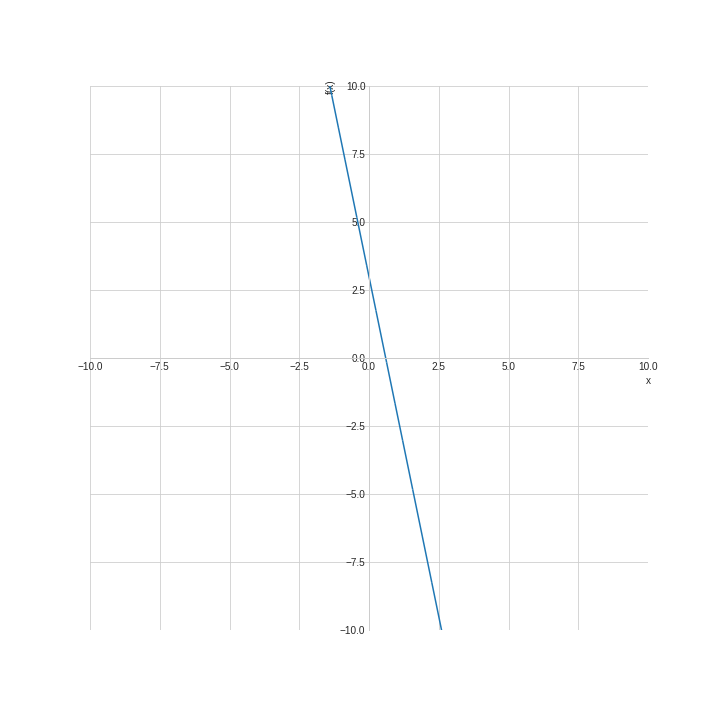
\includegraphics[width=1\columnwidth]{p68e28-1}}   \end{solution} \part[1] $y=x^2-2x-3$  \begin{solution}   \\ \resizebox{0.4\textwidth}{!}{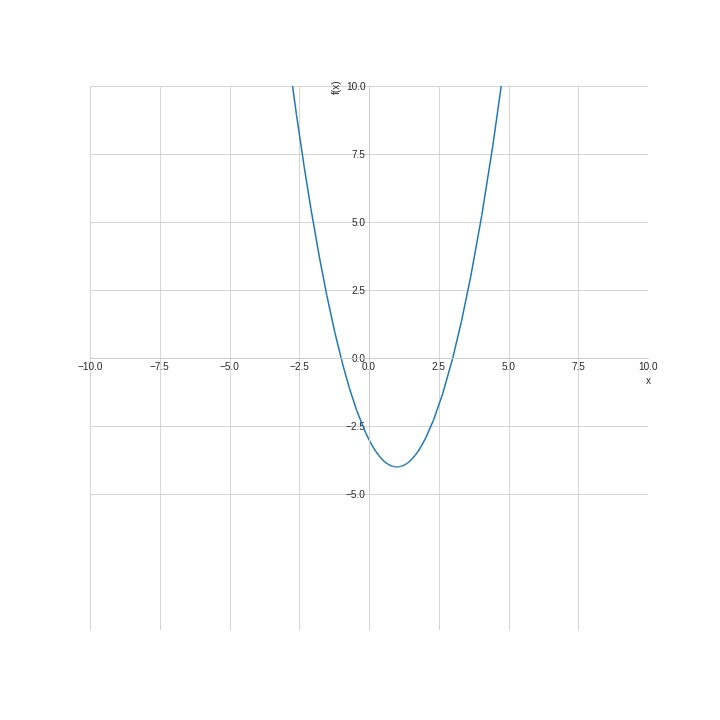
\includegraphics[width=1\columnwidth]{p68e28-2}}   \end{solution} \part[1] $y=4x^2-8x-21$  \begin{solution}   \\ \resizebox{0.4\textwidth}{!}{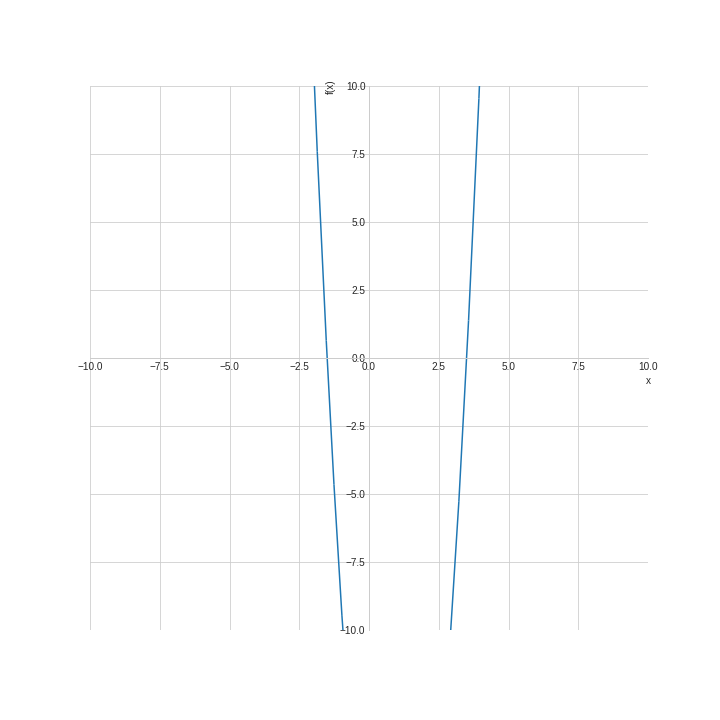
\includegraphics[width=1\columnwidth]{p68e28-3}}   \end{solution}
        \end{parts}
        \end{multicols}
        \question p68e35 - Representa gráficamente las siguientes funciones:
        \begin{multicols}{1}
        \begin{parts} \part[1] $y=\begin{cases} 2 x + 6 & \text{for}\: x < -2 \\x^{2} - 2 & \text{for}\: x \leq -1 \\1 & \text{otherwise} \end{cases}$  \begin{solution}   \\ \resizebox{0.4\textwidth}{!}{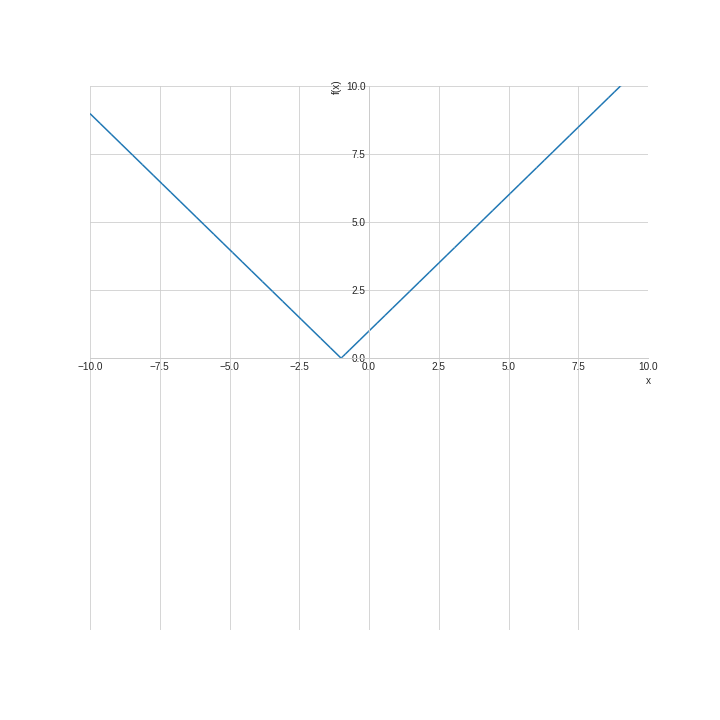
\includegraphics[width=1\columnwidth]{p68e35-0}}   \end{solution} \part[1] $y=\left|{x + 1}\right|$  \begin{solution}   \\ \resizebox{0.4\textwidth}{!}{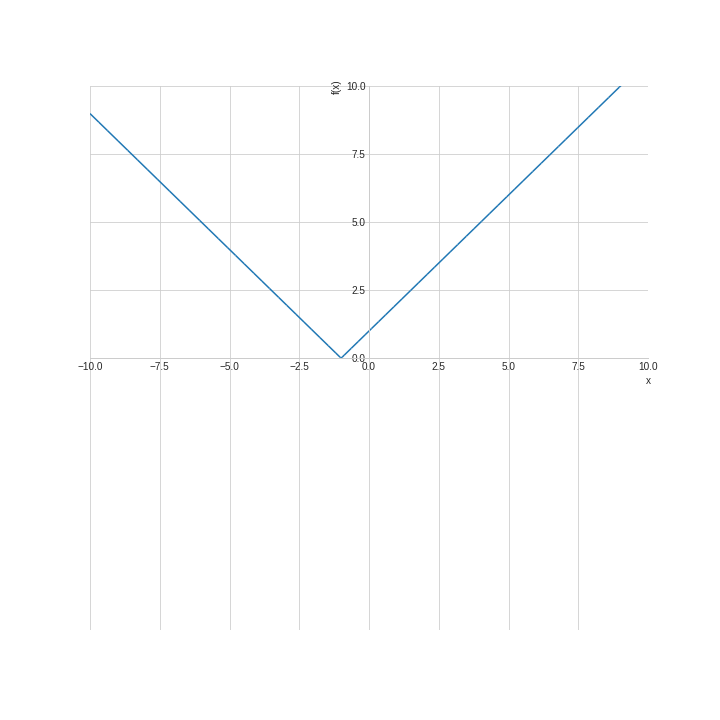
\includegraphics[width=1\columnwidth]{p68e35-1}}   \end{solution} \part[1] $y=\left|{ x^{2} - 2 x - 3}\right|$  \begin{solution}   \\ \resizebox{0.4\textwidth}{!}{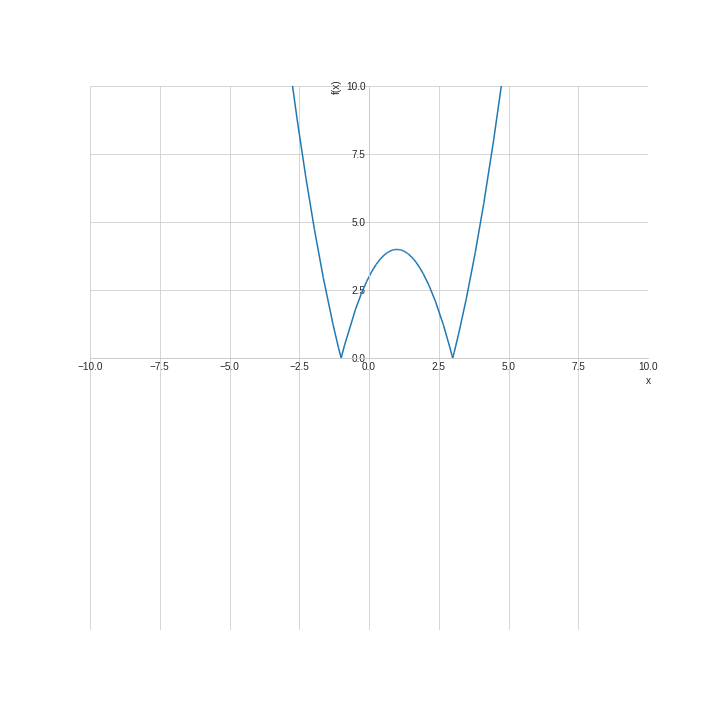
\includegraphics[width=1\columnwidth]{p68e35-2}}   \end{solution} \part[1] $y=\begin{cases} \frac{x}{2} & \text{for}\: x \geq 1 \\\frac{1}{x - 1} & \text{otherwise} \end{cases}$  \begin{solution}   \\ \resizebox{0.4\textwidth}{!}{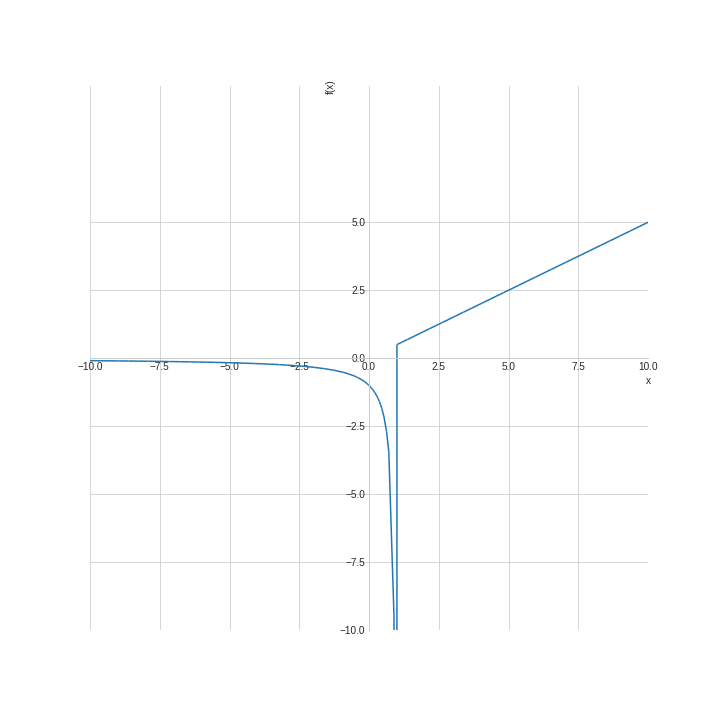
\includegraphics[width=1\columnwidth]{p68e35-3}}   \end{solution}
        \end{parts}
        \end{multicols}
        
    \end{questions}
    \end{document}
    